\section{Complementary-Filtered Residual World Model}

\begin{figure*}[t]
  \centering
  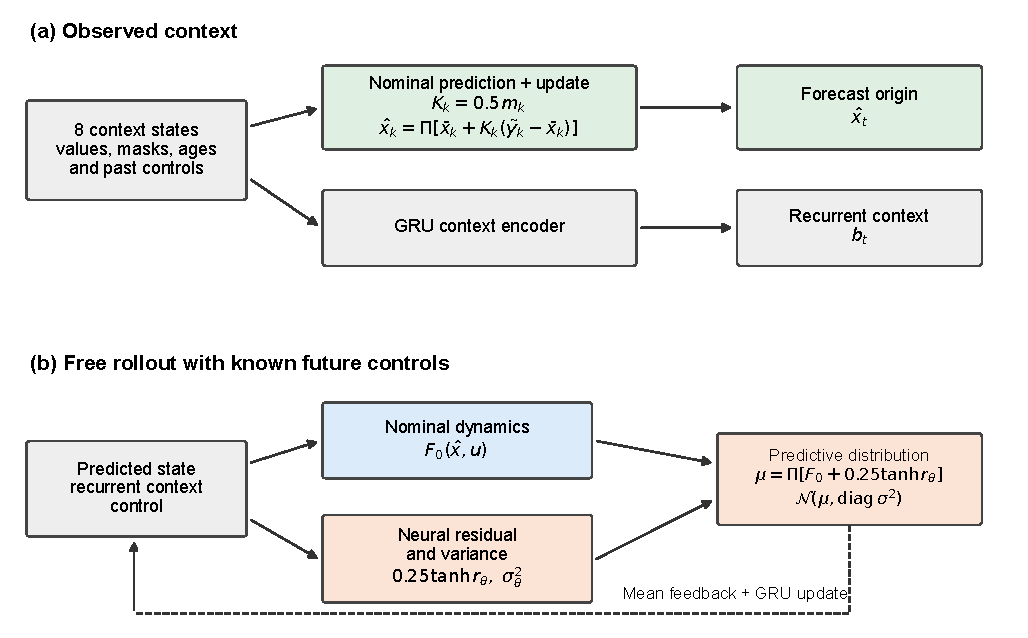
\includegraphics[width=0.92\textwidth]{figures/Fig1.pdf}
  \caption{Causal estimator--predictor interface. Nominal propagation and a
  mask-gated complementary update process the observed context. The corrected
  forecast origin initializes a nominal-plus-residual free rollout under a
  candidate future control sequence. No future observation is used during a
  rollout.}
  \label{fig:method}
\end{figure*}

\subsection{Problem formulation}

Let $\vect{x}_t\in\mathbb{R}^{d_x}$ be a physical state and
$\vect{u}_t\in\mathbb{R}^{d_u}$ a control. The available observation is
\begin{equation}
  \vect{y}_t=\vect{m}_t\odot(\vect{x}_t+\boldsymbol{\epsilon}_t),
\end{equation}
where $\vect{m}_t\in\{0,1\}^{d_x}$ is a channel mask. Missing entries are
filled by the latest available value, giving $\tilde{\vect y}_t$; the mask and
elapsed time since observation $\boldsymbol\delta_t$ remain model inputs.
Given an eight-step context and a candidate future control sequence, the model
predicts $H$ future states without teacher forcing.

\subsection{Mask-gated context update}

Let $F_0$ be a nominal dynamics step. Starting from the first imputed context
state, the filter alternates nominal prediction and measurement correction:
\begin{align}
 \bar{\vect x}_{k} &= F_0(\hat{\vect x}_{k-1},\vect u_{k-1}), \\
 \vect K_k &= \alpha\vect m_k,\qquad \alpha=0.5, \\
 \hat{\vect x}_k &= \Pi\!\left[\bar{\vect x}_k+
 \vect K_k\odot(\tilde{\vect y}_k-\bar{\vect x}_k)\right].
 \label{eq:filter}
\end{align}
An observed channel receives equal pre-projection weight from the nominal
prediction and measurement. A missing channel receives zero direct correction.
$\Pi$ is the identity except for the pendulum sine--cosine representation,
which is projected to the unit circle. The gain is fixed independently of
validation and test outcomes.

A gated recurrent unit (GRU) simultaneously encodes
$[\tilde{\vect y}_k,\vect m_k,\log(1+\boldsymbol\delta_k),\vect u_{k-1}]$.
Its final hidden state carries trajectory context into the rollout, but it does
not alter the measurement gain.

\subsection{Nominal-plus-residual rollout}

At future step $h$, the transition computes
\begin{align}
 \boldsymbol\mu^{p}_{t+h} &= F_0(\hat{\vect x}_{t+h-1},\vect u_{t+h-1}), \\
 [\vect r_{t+h},\vect \ell_{t+h}] &=
 R_\theta([\hat{\vect x}_{t+h-1},\vect u_{t+h-1},\vect b_{t+h-1}]), \\
 \boldsymbol\mu_{t+h} &= \Pi\!\left[
 \boldsymbol\mu^{p}_{t+h}+0.25\tanh(\vect r_{t+h})\right], \\
 \boldsymbol\sigma^2_{t+h} &=
 \max\{\exp(\operatorname{clip}(\vect\ell_{t+h},-8,4)),10^{-6}\}.
 \label{eq:rollout}
\end{align}
The residual is bounded to one quarter of a training standard deviation per
step in normalized coordinates. Predicted means feed the next transition, and
a GRUCell updates $\vect b$. The model minimizes mean diagonal Gaussian
negative log likelihood over all states and all 25 rollout steps:
\begin{equation}
 \mathcal L=\frac{1}{2Hd_x}\sum_{h=1}^{H}\sum_{q=1}^{d_x}
 \left[\log(2\pi\sigma_{hq}^2)+
 \frac{(x_{hq}-\mu_{hq})^2}{\sigma_{hq}^2}\right].
 \label{eq:nll}
\end{equation}

\subsection{Gain and error propagation}

For one observed scalar channel before a nonidentity projection, let
$e_p=\bar x-x$ be nominal prediction error and $\epsilon=y-x$ measurement
error. The filtered error is
$e_f=(1-\alpha)e_p+\alpha\epsilon$. With
$v_p=\mathbb E[e_p^2]$, $v_\epsilon=\mathbb E[\epsilon^2]$, and
$c=\mathbb E[e_p\epsilon]$,
\begin{equation}
 \mathbb E[e_f^2]=(1-\alpha)^2v_p+\alpha^2v_\epsilon
 +2\alpha(1-\alpha)c.
 \label{eq:mse}
\end{equation}
If $v_p+v_\epsilon-2c>0$, its constrained minimizer is
\begin{equation}
 \alpha^*=\operatorname{clip}_{[0,1]}
 \left(\frac{v_p-c}{v_p+v_\epsilon-2c}\right).
 \label{eq:alpha}
\end{equation}
Thus $\alpha=0.5$ is optimal only when $v_p=v_\epsilon$ and $c=0$. This
identity predicts regime dependence: cleaner measurements favor a larger gain,
whereas inaccurate nominal propagation favors stronger measurement correction.

If the rollout transition is locally $L$-Lipschitz with local error $\eta_h$,
\begin{equation}
 \|\hat{\vect x}_{t+H}-\vect x_{t+H}\|
 \le L^H\|\hat{\vect x}_t-\vect x_t\|
 +\sum_{h=0}^{H-1}L^{H-1-h}\eta_h.
 \label{eq:rollout_bound}
\end{equation}
The filter changes the initial-error term; the residual changes the accumulated
transition term. The component experiments estimate their separate effects.

\subsection{Receding-horizon use}

For each control step, the current eight-state context is processed once per
candidate sequence. Cross-entropy MPC samples bounded action sequences,
evaluates their predicted mean trajectories, retains the lowest-cost elites,
and applies the first action of the updated mean. The next optimization is warm
started by shifting that mean. The model is not retrained for the control
objective, and predictive variances are not used by this controller.

